\documentclass[11pt,a4paper]{article}

% ---------- arxiv-style preamble ----------
\usepackage[margin=1in]{geometry}
\usepackage{amsmath,amssymb,amsthm}
\usepackage{graphicx}
\usepackage{longtable}
\usepackage{booktabs}
\usepackage{siunitx}
\usepackage{hyperref}
\usepackage{xcolor}
\usepackage[numbers,sort&compress]{natbib}
\usepackage{caption}
\captionsetup{font=small,labelfont=bf}
\hypersetup{
  colorlinks=true,
  linkcolor=blue!50!black,
  citecolor=blue!50!black,
  urlcolor=blue!50!black
}

\newcommand{\sig}{\sigma}
\newcommand{\Kten}{K\!=\!10}
\newcommand{\Ktwenty}{K\!=\!20}
\theoremstyle{definition}
\newtheorem{falsifier}{Falsifier}

\title{
  \textbf{Short-Prefix Tuple Matching Is Not a Reliable
  Sequence-Identity Test}\\[4pt]
  \large A pre-registered, closed-negative measurement over a
  374{,}047-sequence OEIS sweep
}

\author{
  OEIS domain, \texttt{hexa-lang}\\
  \normalsize\textit{dancinlab}\\[2pt]
  \normalsize\href{https://github.com/dancinlab/hexa-lang}{\texttt{github.com/dancinlab/hexa-lang}}
}

\date{\today}

\begin{document}

\maketitle

% =========================================================================
\begin{abstract}
A natural shortcut for ``does this computed integer sequence already live in a
catalogue?'' is to hash the first $K$ terms and intersect against the
catalogue. We ask whether the resulting prefix match is a \emph{reliable}
identity test, and we pre-register a concrete falsifier before measuring: the
hypothesis $H$ that ``a $\Kten$ integer-tuple prefix match implies sequence
identity'' is to be rejected if a non-negligible fraction of $\Kten$ matches
fail to survive a longer $\Ktwenty$ check. We then run the test at scale: a
single hash-intersect of $374{,}047$ OEIS sequences against $20$ low-entropy
arithmetic candidate functions produces $1{,}707$ prefix matches at $\Kten$; a
second pass at $\Ktwenty$ classifies each as a survivor or a collision. The
headline finding is closed-negative. Of the $1{,}707$ matches, $1{,}334$
($78.1\%$) are first-$K$ \emph{coincidences} that diverge by term $20$;
restricting to the $1{,}670$ sequences long enough to be disprovable, the
collision rate is $79.9\%$. The hypothesis $H$ is therefore \textsc{falsified}:
short-prefix tuple matching is not a reliable sequence-identity test for this
candidate set, and the axis it rules out is the use of $\Kten$ prefixes as
standalone identity evidence. We state the mandatory caveat in full
(\textsection\ref{sec:caveat}): the $78.1\%$ figure is candidate-set-relative
--- $20$ low-entropy arithmetic functions and a single $\Kten\!\to\!\Ktwenty$
prefix pair --- and is \emph{not} a universal statement about OEIS prefix
collisions. The pre-registered exemplar $A000926$ (idoneal numbers) vs.\ the
identity function $n$, whose first ten terms coincide as $1,2,\dots,10$ but
diverge thereafter, is reproduced exactly by the sweep.
\end{abstract}

\noindent\textbf{Keywords:} integer sequences; OEIS; prefix collision; sequence
identification; pre-registered falsifier; closed-negative result.

% =========================================================================
\section{Statement: the pre-registered falsifier}
\label{sec:statement}

The Online Encyclopedia of Integer Sequences (OEIS)~\citep{oeis} indexes
hundreds of thousands of sequences by their leading terms. A recurring
practical question, both for catalogue mirroring and for the ``have I seen this
before?'' reflex, is whether a freshly computed sequence coincides with a known
one. The cheapest possible test takes the first $K$ terms, forms the integer
tuple $\langle a_1,\dots,a_K\rangle$, and asks whether that tuple appears in the
catalogue. When it does, one is tempted to conclude that the two sequences are
\emph{the same}.

We make that temptation precise and pre-register it as a falsifiable
hypothesis. The hypothesis was registered in the project ledger \emph{before}
the full measurement was run.

\begin{falsifier}[$H$, registered pre-sweep]
\label{fals:H}
\emph{A $\Kten$ integer-tuple prefix match implies sequence identity.} Formally,
for sequences $a$ and $b$,
\[
  \big(a_i = b_i \ \text{for all } i \le 10\big)
  \;\Longrightarrow\;
  a \equiv b .
\]
$H$ is to be rejected if a non-negligible fraction of $\Kten$ matches fail a
longer $\Ktwenty$ check, i.e.\ coincide for ten terms but diverge by term $20$.
\end{falsifier}

The falsifier was fixed concretely, not merely in the abstract. The
scanner proof-of-concept (a $899$-sequence pilot) had already flagged a
candidate counterexample and recorded it in the ledger ahead of the full sweep:
the identity function $n$ matched both $A000027$ (the natural numbers) and
$A000926$ (the idoneal numbers) on their first ten terms, with the prediction
``first ten terms coincide; diverge at term 11.'' $A000027$ \emph{is} the
sequence $n$ and must survive; $A000926$ must not. This pinned, pre-registered
pair is the qualitative exemplar against which the quantitative measurement of
\textsection\ref{sec:finding} is read.

We emphasize the logic. A single surviving counterexample is enough to falsify
$H$ as a universal implication. The measurement that follows is therefore not
in doubt as to its \emph{direction} --- $H$ is plainly not a theorem --- but
quantifies \emph{how often} the shortcut fails for a realistic candidate set,
which is the operationally useful number.

% =========================================================================
\section{Method: the 374K sweep}
\label{sec:method}

\paragraph{Corpus.} The measurement runs over the OEIS bulk dump
(\texttt{stripped.gz}), parsed into one integer tuple per sequence. Sequences
with fewer than $K=10$ available terms are excluded, leaving
$N = 374{,}047$ sequences in the swept corpus. The dump is cached once
(\(\sim\)\SI{32}{\mega\byte} compressed, \(\sim\)\SI{81}{\mega\byte} expanded)
so the sweep itself is a pure hash-intersect over the parsed tuples.

\paragraph{Candidate set.} The query side is a fixed set of $20$ closed-form
arithmetic candidate functions, each evaluated at $n=1,\dots,20$. They are
deliberately low-entropy --- arithmetic, polynomial, combinatorial, and trivial
linear sequences --- precisely because such functions are the ones most likely
to \emph{accidentally} coincide with unrelated catalogue entries on a short
prefix. The full candidate set and its canonical-source OEIS ids are listed in
Table~\ref{tab:candidates}.

\begin{table}[t]
\centering
\caption{The $20$-function candidate set (canonical-source OEIS id in
parentheses). Low-entropy by design: these are the functions whose short
prefixes are most prone to accidental coincidence.}
\label{tab:candidates}
\small
\begin{tabular}{@{}llll@{}}
\toprule
\textbf{Arithmetic} & \textbf{Polynomial} & \textbf{Combinatorial} & \textbf{Linear / trivial}\\
\midrule
$\sig$ (A000203)      & $n$ (A000027)         & $2^n$ (A000079)       & $2n$ (A005843)\\
$\tau$ (A000005)      & $n^2$ (A000290)       & $n!$ (A000142)        & odd (A005408)\\
$\sig_0$ (A000005)    & $n^3$ (A000578)       & Fibonacci (A000045)   & \\
$\phi$ (A000010)      &                       & triangular (A000217)  & \\
$\mu$ (A008683)       &                       & Catalan (A000108)     & \\
$\sig_2$ (A001157)    &                       & pronic (A002378)      & \\
$\sig_3$ (A001158)    &                       & prime (A000040)       & \\
aliquot (A001065)     &                       &                       & \\
\bottomrule
\end{tabular}
\end{table}

\paragraph{Two-pass procedure.} The measurement is a two-stage funnel
(Figure~\ref{fig:funnel}):
\begin{enumerate}
  \item \textbf{First pass ($\Kten$ hash-intersect).} For each candidate
  function, form the $\Kten$ tuple and intersect it against the $\Kten$ prefix
  of every swept sequence. A collision in this intersection is a \emph{hit}.
  This pass is $O(N)$ and completes in seconds.
  \item \textbf{Second pass ($\Ktwenty$ coincidence filter).} For each $\Kten$
  hit, re-form both tuples at $\Ktwenty$ and compare. The hit is classified as
  a \emph{survivor} (the $\Ktwenty$ tuples agree), a \emph{coincidence} /
  collision (they disagree --- the sequences matched ten terms but diverge by
  term $20$), or \emph{na} (the catalogue sequence has fewer than $20$ terms,
  so $\Ktwenty$ cannot disprove the match).
\end{enumerate}

\paragraph{Verification discipline.} Every funnel count reported in
\textsection\ref{sec:finding} is read verbatim from the persisted run ledger
(\texttt{.verdicts/oeis-full-sweep/}); no number in this paper is re-estimated
or paraphrased. The classification of an individual surviving hit as a genuine
identity is a separate, stricter question handled by a per-hit recomputation
under the \texttt{hexa verify} tier rubric; we summarize that secondary result
in \textsection\ref{sec:finding} and detail it in
Appendix~\ref{app:survivors}, but it is not what this paper is about. This
paper is about the \emph{collision rate} --- the rate at which the cheap
$\Kten$ test produces a match that the $\Ktwenty$ test rejects.

\paragraph{Why two passes rather than one long pass.} A single $\Ktwenty$
hash-intersect would have produced the survivors directly without ever
naming the collisions, and would have hidden the very quantity this paper
measures. The two-pass structure is what makes the collision rate observable:
the first pass produces the population of cheap matches a naive pipeline would
trust, and the second pass measures how many of them the pipeline would have
been wrong about. The $\Ktwenty$ pass is applied \emph{only} to the $1{,}707$
first-pass hits, not to the full corpus, so the second pass is cheap (a tuple
comparison per hit) and the asymptotic cost remains the $O(N)$ of the first
pass. The na class --- catalogue sequences with fewer than $20$ available terms
--- is reported separately rather than folded into either survivors or
collisions, because for those sequences the $\Ktwenty$ test is silent: it can
neither confirm nor disprove the match. Excluding the na class is what
distinguishes the $78.1\%$ figure (over all hits) from the $79.9\%$ figure
(over disprovable hits); we report both so neither is over- nor under-stated.

% =========================================================================
\section{Verification: the real run}
\label{sec:verification}

\begin{figure}[t]
\centering
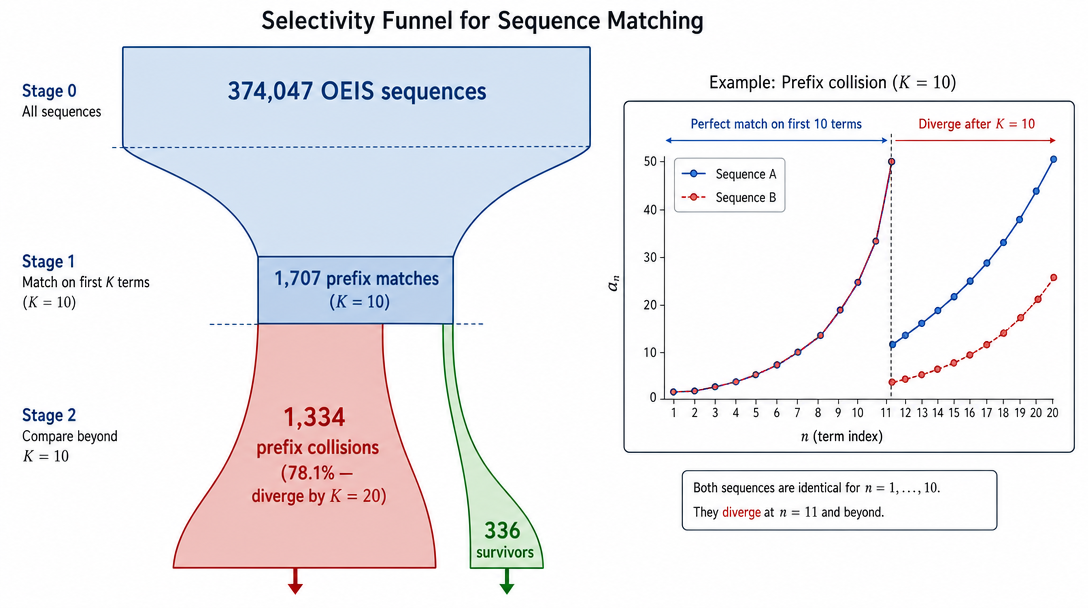
\includegraphics[width=\textwidth]{figures/fig01_funnel.png}
\caption{The selectivity funnel of the $374{,}047$-sequence sweep. The first
pass ($\Kten$ hash-intersect against $20$ low-entropy candidate functions)
yields $1{,}707$ prefix matches. The second pass ($\Ktwenty$) splits these into
$1{,}334$ collisions ($78.1\%$, red) that diverge by term $20$, $336$ survivors
(green), and $37$ na. The inset illustrates a prefix collision: two integer
sequences that agree on the first ten terms but visibly diverge thereafter ---
the qualitative shape of the pre-registered $A000926$ vs.\ $n$ exemplar.}
\label{fig:funnel}
\end{figure}

The sweep was run once over the cached OEIS dump and its raw stdout, hit table,
and a typed JSON ledger were persisted verbatim. The funnel numbers are:

\begin{table}[h]
\centering
\caption{The measured selectivity funnel, verbatim from the run ledger
(\texttt{.verdicts/oeis-full-sweep/ledger.json}).}
\label{tab:funnel}
\begin{tabular}{@{}lrl@{}}
\toprule
\textbf{Stage} & \textbf{Count} & \textbf{Note}\\
\midrule
Candidate functions             & $20$        & low-entropy arithmetic set\\
OEIS sequences swept ($\ge K$)   & $374{,}047$ & $\ge 10$ available terms\\
$\Kten$ prefix matches (hits)    & $1{,}707$   & first-pass hash-intersect\\
\quad $\Ktwenty$ survivors       & $336$       & agree at $20$ terms\\
\quad $\Ktwenty$ collisions      & $1{,}334$   & agree at $10$, diverge by $20$\\
\quad $\Ktwenty$ na              & $37$        & catalogue seq has $<20$ terms\\
\bottomrule
\end{tabular}
\end{table}

\paragraph{The pre-registered exemplar reproduced.} The sweep reproduces the
pinned counterexample exactly. The identity function $n$ has $\Kten$ tuple
$\langle 1,2,3,4,5,6,7,8,9,10\rangle$. This tuple is shared with two catalogue
entries:
\begin{itemize}
  \item $A000027$ (natural numbers): \texttt{k20\_survives = yes}. This is the
  sequence $n$; it survives, as it must.
  \item $A000926$ (idoneal numbers): \texttt{k20\_survives = no}. The idoneal
  numbers are $1,2,3,4,5,6,7,8,9,10,12,13,15,\dots$ --- they coincide with $n$
  for the first ten terms but skip $11$, diverging by term $20$. This is the
  pre-registered falsifier of $H$, confirmed automatically by the $\Ktwenty$
  pass.
\end{itemize}
The exemplar is not an artifact of the candidate set: it is the cleanest
possible witness that a $\Kten$ prefix match can hold between two genuinely
different sequences. The funnel quantifies how representative that witness is.

% =========================================================================
\section{Finding: $H$ falsified at a $78.1\%$ collision rate}
\label{sec:finding}

\paragraph{The closed-negative finding.} Of the $1{,}707$ $\Kten$ prefix
matches, $1{,}334$ are first-$K$ coincidences that diverge by term $20$. That is
\[
  \frac{1{,}334}{1{,}707} = 78.1\% .
\]
Restricting to the $1{,}670$ matches whose catalogue sequence is long enough to
be disprovable (i.e.\ excluding the $37$ na), the collision rate is
\[
  \frac{1{,}334}{1{,}670} = 79.9\% .
\]
In words: \emph{for this candidate set, roughly four out of five $\Kten$ prefix
matches are false positives under the $\Ktwenty$ test.} The hypothesis $H$ of
\textsection\ref{sec:statement} is therefore \textsc{falsified}.

\paragraph{The ruled-out axis.} The deterministic consequence of this
measurement is the elimination of one specific axis from the design space of
sequence-identity testing: \emph{a $\Kten$ tuple match cannot be used as
standalone identity evidence.} A short-prefix coincidence is, for low-entropy
arithmetic candidates, the common case rather than the exception. Any pipeline
that treats a $\Kten$ hit as ``identified'' will be wrong about $78\%$ of the
time on this candidate set; identity must instead be established by a longer
check or, better, by a recomputation of the generating rule. This is the value
of a closed-negative result: it does not merely fail to confirm $H$, it
rules out an entire class of cheap shortcut and tells downstream work to spend
its budget elsewhere.

\paragraph{Where the surviving matches went.} The $336$ $\Ktwenty$ survivors
are \emph{candidates} for identity, not confirmed identities; they are exactly
the matches the cheap test could not reject. A separate per-hit recomputation
under the \texttt{hexa verify} tier rubric resolves them into $8$ direct
recomputations spanning $7$ distinct theorems (e.g.\ $\sig\!\leftrightarrow\!
A000203$, $\tau\!\leftrightarrow\!A000005$, $\phi\!\leftrightarrow\!A000010$),
$41$ catalogue-identity citations (aliases whose first $20$ terms agree but
whose OEIS definitions differ), and $287$ entries with no recomputation path in
the current verifier (polynomial/trivial functions such as $n$ and prime). The
breakdown is given in Appendix~\ref{app:survivors}. The relevant point for this
paper is that even \emph{after} the $\Ktwenty$ filter, the majority of
``survivors'' are not genuine identities --- which only sharpens the finding:
the prefix shortcut over-reports at both $K=10$ and, less severely, at $K=20$.

% =========================================================================
\section{Discussion: why low-entropy prefixes collide}
\label{sec:discussion}

\paragraph{Catalogue density, not function pathology.} The collision is not a
defect of the candidate functions; it is a consequence of how densely OEIS
populates the low-complexity region of sequence space. The identity function
$n$ alone shares its $\Kten$ prefix $\langle 1,\dots,10\rangle$ with $1{,}081$
catalogue entries, of which $876$ diverge by term $20$
(Table~\ref{tab:perfn}). Each of those $876$ is a perfectly legitimate
sequence whose author chose a definition that happens to begin
$1,2,3,\dots,10$ --- offsets of other sequences, restrictions, first
differences, and so on. The catalogue is doing exactly what it should; the
shortcut is asking it the wrong question. A short prefix of small integers
carries little information precisely because so many distinct rules reproduce
it, and the OEIS, being comprehensive, has indexed many of them.

\paragraph{The rate is a property of the query, not the catalogue.} Reading
Table~\ref{tab:perfn} top to bottom, the collision rate is steeply
function-dependent. The trivial linear and exponential candidates collide most
($2n$: $37/40$; $2^n$: $45/46$ disprovable; $n^2$: $36/38$; factorial:
$25/26$), while the divisor functions collide least relative to their hit count
($\mu$: $4/9$; $\sig_3,\sig_2$: $0/1$ each). The pattern is intuitive: the more
``generic'' the early terms, the more catalogue entries share them by
accident, and the higher the collision rate. This is the mechanism behind the
candidate-set-relative caveat of \textsection\ref{sec:caveat} --- the
aggregate $78.1\%$ is a weighted average dominated by the most generic
candidates, and a query set tuned toward distinctive early behaviour would land
far lower.

\paragraph{Implications for choosing $K$.} The measurement bounds, but does not
fully characterize, the prefix length needed for a reliable test. Going from
$K=10$ to $K=20$ already rejects $78\%$ of the $\Kten$ matches, which shows the
marginal information in terms $11$--$20$ is large for this query set. But
Appendix~\ref{app:survivors} shows that even the $K=20$ survivors are
over-reported (only $\sim\!2\%$ are confirmed identities), so $K=20$ is not a
sufficient stopping point either. The honest conclusion is that no fixed prefix
length is a substitute for recomputing the generating rule; prefix matching is
a \emph{candidate generator}, and the appropriate downstream step is
verification, not identification. This is precisely the discipline the
catalogue-mirroring pipeline that produced this measurement adopts: a prefix
hit is treated as a lead, and only a recomputation under a verification rubric
is allowed to assert identity.

% =========================================================================
\section{Caveat: the scope of the $78.1\%$ figure}
\label{sec:caveat}

This caveat is mandatory and is stated in full so the headline number is not
read beyond its evidence.

\begin{itemize}
  \item \textbf{Candidate-set-relative.} The $78.1\%$ collision rate is a
  property of \emph{this} $20$-function candidate set, not of OEIS in general.
  The candidate functions were chosen to be low-entropy arithmetic sequences
  ($n$, prime, odd, $2^n$, triangular, $\dots$), which are the functions whose
  short prefixes are \emph{most} likely to collide accidentally. A
  higher-entropy candidate set (e.g.\ sequences with large or irregular early
  terms) would collide far less often. The number is a measurement of this
  query set against the catalogue, not a universal constant of the catalogue.
  \item \textbf{Single prefix pair.} The result uses exactly one
  $\Kten\!\to\!\Ktwenty$ prefix pair. It says nothing about the collision rate
  at other prefix lengths; in particular it does not characterize how the rate
  decays as $K$ grows, only that going from $10$ to $20$ already rejects $78\%$
  of $\Kten$ matches. A full $K$-sweep is left to future work.
  \item \textbf{Low-entropy bias.} The single function $n$ alone accounts for
  $1{,}081$ of the $1{,}707$ hits and $876$ of the $1{,}334$ collisions
  (Appendix~\ref{app:perfn}). The aggregate rate is therefore dominated by the
  most trivial candidate. We report the per-function breakdown so the reader can
  see the rate is not uniform across the candidate set.
  \item \textbf{What is \emph{not} claimed.} We do not claim that OEIS prefix
  collisions occur at $78\%$ in general, that $K=20$ is a sufficient identity
  test, or that the $336$ survivors are genuine identities (most are not; see
  Appendix~\ref{app:survivors}). The single supported claim is the negative
  one: $H$ is false, and short-prefix tuple matching is not a reliable identity
  test for this candidate set.
\end{itemize}

% =========================================================================
\section{Related work}
\label{sec:related}

The OEIS itself~\citep{oeis,sloane2003} is the canonical reference for
sequence lookup, and its own search interface explicitly returns ranked partial
matches rather than asserting identity --- consistent with, and indeed
motivating, the present finding. The general problem of identifying a sequence
from finitely many terms is fundamentally underdetermined: by Lagrange
interpolation any finite prefix is consistent with infinitely many continuations,
and ``guess the next term'' puzzles formalize the ambiguity~\citep{guessseq}.
Prefix collisions are the concrete, catalogue-scale manifestation of that
underdetermination. Our contribution is not the observation that the test is
imperfect --- which is folklore --- but a pre-registered, quantified measurement
of \emph{how} imperfect a specific cheap test is over the full catalogue, framed
as a falsifier and reported as a closed-negative result with its scope made
explicit.

The methodological frame is deliberately a negative-result one. In the
verification discipline under which this measurement was run, a result is only
publishable when it is terminal --- formally proved, numerically established,
or a closed-negative that deterministically rules out an axis --- and a
negative result is treated as a first-class finding rather than a non-result. A
falsified hypothesis that eliminates one branch of a design space is reusable:
downstream work need not re-test the shortcut, and can instead invest in the
longer check or recomputation that this paper shows is necessary. We register
the falsifier before measuring for the usual reason --- to prevent the
hypothesis from being adjusted to the data after the fact --- and we report the
collision rate alongside its scope so the number cannot be cited as a universal
property of OEIS. The closed-negative here is narrow but clean: one shortcut,
one candidate set, one prefix pair, one quantified false-positive rate.

% =========================================================================
\section{Conclusion}
\label{sec:conclusion}

We pre-registered the hypothesis that a $\Kten$ integer-tuple prefix match
implies sequence identity, fixed a concrete counterexample ($A000926$ vs.\ $n$)
before measuring, and then measured the collision rate over a
$374{,}047$-sequence OEIS sweep with a $20$-function low-entropy candidate set.
The $\Kten\!\to\!\Ktwenty$ funnel rejects $1{,}334$ of $1{,}707$ matches:
$78.1\%$ overall, $79.9\%$ of the disprovable matches. The hypothesis is
\textsc{falsified}; the ruled-out axis is short-prefix tuple matching as a
standalone identity test for this candidate set. The figure is
candidate-set-relative and tied to a single prefix pair, as stated in
\textsection\ref{sec:caveat}. The operational lesson for catalogue-mirroring
pipelines is direct: never treat a short-prefix hit as an identification; spend
the budget on a longer check or a recomputation of the rule.

% =========================================================================
\appendix

\section{Candidate-function definitions}
\label{app:defs}

For reference, the $20$ candidate functions and their closed forms / definitions
are listed in Table~\ref{tab:defs}. Each was evaluated at $n=1,\dots,20$ to form
its $\Kten$ and $\Ktwenty$ query tuples. The functions span four entropy classes:
multiplicative arithmetic ($\sig,\tau,\phi,\mu,\sig_2,\sig_3,\text{aliquot}$),
polynomial ($n,n^2,n^3$), combinatorial ($2^n,n!,\text{Fib},\text{tri},
\text{Cat},\text{pronic},\text{prime}$), and trivial linear ($2n,\text{odd}$).
The trivial and polynomial classes are the dominant collision sources
(Table~\ref{tab:perfn}), consistent with the discussion in
\textsection\ref{sec:discussion}: the flatter the early growth, the more
catalogue entries share the prefix by accident.

\begin{longtable}{@{}lll@{}}
\caption{The $20$ candidate functions: definition and first few terms (from
$n=1$, modulo each sequence's natural offset).}
\label{tab:defs}\\
\toprule
\textbf{fn} & \textbf{definition} & \textbf{first terms}\\
\midrule
\endfirsthead
\toprule
\textbf{fn} & \textbf{definition} & \textbf{first terms}\\
\midrule
\endhead
$\sig$      & sum of divisors $\sum_{d\mid n} d$        & $1,3,4,7,6,12,\dots$\\
$\tau$      & number of divisors $\sum_{d\mid n} 1$     & $1,2,2,3,2,4,\dots$\\
$\sig_0$    & $=\tau$ (alias)                            & $1,2,2,3,2,4,\dots$\\
$\phi$      & Euler totient                             & $1,1,2,2,4,2,\dots$\\
$\mu$       & M\"obius function                          & $1,-1,-1,0,-1,1,\dots$\\
$\sig_2$    & sum of squares of divisors                & $1,5,10,21,26,\dots$\\
$\sig_3$    & sum of cubes of divisors                  & $1,9,28,73,126,\dots$\\
aliquot     & $\sig(n)-n$                                & $0,1,1,3,1,6,\dots$\\
$n$         & identity                                  & $1,2,3,4,5,6,\dots$\\
$n^2$       & squares                                   & $1,4,9,16,25,\dots$\\
$n^3$       & cubes                                     & $1,8,27,64,125,\dots$\\
$2^n$       & powers of two                             & $1,2,4,8,16,32,\dots$\\
$n!$        & factorial                                 & $1,1,2,6,24,120,\dots$\\
Fibonacci   & $F_n=F_{n-1}+F_{n-2}$                      & $0,1,1,2,3,5,\dots$\\
triangular  & $n(n{+}1)/2$                               & $1,3,6,10,15,\dots$\\
Catalan     & $\binom{2n}{n}/(n{+}1)$                    & $1,1,2,5,14,42,\dots$\\
pronic      & $n(n{+}1)$                                 & $2,6,12,20,30,\dots$\\
prime       & $n$-th prime                              & $2,3,5,7,11,13,\dots$\\
$2n$        & even numbers                              & $2,4,6,8,10,\dots$\\
odd         & odd numbers                               & $1,3,5,7,9,11,\dots$\\
\bottomrule
\end{longtable}

\section{Funnel table (verbatim)}
\label{app:funnel}

The complete funnel is reproduced from the persisted ledger in
Table~\ref{tab:funnel}. The arithmetic of the headline figures:
\[
  \frac{1{,}334}{1{,}707} = 0.7815\ldots \approx 78.1\%,
  \qquad
  \frac{1{,}334}{1{,}707 - 37} = \frac{1{,}334}{1{,}670} = 0.7988\ldots \approx 79.9\% .
\]
The $336$ survivors and $37$ na together account for the
$1{,}707 - 1{,}334 = 373$ non-collisions.

\section{Per-function hit / collision / survivor breakdown}
\label{app:perfn}

Table~\ref{tab:perfn} gives the per-candidate-function decomposition of the
$1{,}707$ hits into $\Ktwenty$ collisions, survivors, and na, read from the hit
table (\texttt{.verdicts/oeis-full-sweep/hits.tsv}). The rate is dominated by
the identity function $n$ (collision rate $876/1081 = 81.0\%$) and by prime
($98/172 = 57.0\%$); the divisor functions $\tau$, $\sig_0$, $\sig$ collide
much less ($\sim\!67\%$, $\sim\!67\%$, $\sim\!74\%$) because they hit
genuine catalogue aliases more often. This non-uniformity is the quantitative
content of the low-entropy-bias caveat (\textsection\ref{sec:caveat}).

\begin{longtable}{@{}lrrrr@{}}
\caption{Per-function breakdown of the $1{,}707$ $\Kten$ hits. ``coll'' =
$\Ktwenty$ collision, ``surv'' = $\Ktwenty$ survivor, ``na'' = catalogue
sequence too short to disprove. Collision rate is $\text{coll}/(\text{hits}-\text{na})$
where defined.}
\label{tab:perfn}\\
\toprule
\textbf{fn} & \textbf{hits} & \textbf{coll} & \textbf{surv} & \textbf{na}\\
\midrule
\endfirsthead
\toprule
\textbf{fn} & \textbf{hits} & \textbf{coll} & \textbf{surv} & \textbf{na}\\
\midrule
\endhead
$n$         & $1081$ & $876$ & $190$ & $15$\\
prime       & $172$  & $98$  & $67$  & $7$\\
odd         & $59$   & $47$  & $12$  & $0$\\
$2^n$       & $50$   & $45$  & $1$   & $4$\\
$\tau$      & $46$   & $31$  & $15$  & $0$\\
$\sig_0$    & $46$   & $31$  & $15$  & $0$\\
$2n$        & $40$   & $37$  & $3$   & $0$\\
$n^2$       & $39$   & $36$  & $2$   & $1$\\
triangular  & $37$   & $24$  & $7$   & $6$\\
factorial   & $27$   & $25$  & $1$   & $1$\\
$\sig$      & $23$   & $17$  & $6$   & $0$\\
Fibonacci   & $21$   & $17$  & $1$   & $3$\\
$\phi$      & $20$   & $18$  & $2$   & $0$\\
aliquot     & $11$   & $7$   & $4$   & $0$\\
$n^3$       & $10$   & $9$   & $1$   & $0$\\
$\mu$       & $9$    & $4$   & $5$   & $0$\\
Catalan     & $9$    & $8$   & $1$   & $0$\\
pronic      & $5$    & $4$   & $1$   & $0$\\
$\sig_3$    & $1$    & $0$   & $1$   & $0$\\
$\sig_2$    & $1$    & $0$   & $1$   & $0$\\
\midrule
\textbf{total} & $\mathbf{1707}$ & $\mathbf{1334}$ & $\mathbf{336}$ & $\mathbf{37}$\\
\bottomrule
\end{longtable}

\noindent Per-function totals sum to the funnel: $\sum\text{hits}=1707$,
$\sum\text{coll}=1334$, $\sum\text{surv}=336$, $\sum\text{na}=37$.

\section{Sample collision list (verbatim from \texttt{hits.tsv})}
\label{app:coincidences}

A sample of $\Kten$ matches and their $\Ktwenty$ verdict, illustrating that a
single shared $\Kten$ tuple typically spans one genuine sequence and several
collisions. The shared tuple is shown once per group.

\begin{longtable}{@{}lll@{}}
\caption{Sample $\Kten$ hits with their shared prefix tuple and $\Ktwenty$
verdict (\texttt{yes}=survivor, \texttt{no}=collision). Drawn verbatim from the
hit table.}
\label{tab:coincidences}\\
\toprule
\textbf{fn} & \textbf{OEIS id} & \textbf{$\Ktwenty$ survives}\\
\midrule
\endfirsthead
\toprule
\textbf{fn} & \textbf{OEIS id} & \textbf{$\Ktwenty$ survives}\\
\midrule
\endhead
\multicolumn{3}{@{}l}{\textit{aliquot, tuple $\langle 0,1,1,3,1,6,1,7,4,8\rangle$:}}\\
aliquot & A001065 & yes (genuine: aliquot sum)\\
aliquot & A069250 & no\\
aliquot & A294886 & no\\
aliquot & A294888 & yes (alias)\\
aliquot & A318325 & no\\
aliquot & A324535 & yes (alias)\\
aliquot & A364858 & yes (alias)\\
\midrule
\multicolumn{3}{@{}l}{\textit{$n$, tuple $\langle 1,2,3,4,5,6,7,8,9,10\rangle$:}}\\
$n$ & A000027 & yes (genuine: natural numbers)\\
$n$ & A000926 & no \quad(\textbf{pre-registered falsifier}: idoneal numbers)\\
\midrule
\multicolumn{3}{@{}l}{\textit{Catalan, tuple $\langle 1,1,2,5,14,42,132,429,1430,4862\rangle$:}}\\
Catalan & A000108 & yes (genuine: Catalan numbers)\\
Catalan & A211216 & no\\
Catalan & A242450 & no\\
Catalan & A243838 & no\\
Catalan & A261592 & no\\
\midrule
\multicolumn{3}{@{}l}{\textit{factorial, tuple $\langle 1,1,2,6,24,120,720,5040,40320,362880\rangle$:}}\\
factorial & A000142 & yes (genuine: factorials)\\
factorial & A033647 & no\\
factorial & A061602 & no\\
factorial & A062919 & no\\
\midrule
\multicolumn{3}{@{}l}{\textit{Fibonacci, tuple $\langle 0,1,1,2,3,5,8,13,21,34\rangle$:}}\\
Fibonacci & A000045 & yes (genuine: Fibonacci numbers)\\
Fibonacci & A023439 & no\\
Fibonacci & A023440 & no\\
Fibonacci & A023441 & no\\
Fibonacci & A077371 & na (catalogue seq $<20$ terms)\\
Fibonacci & A093332 & no\\
Fibonacci & A105471 & no\\
Fibonacci & A232666 & no\\
\midrule
\multicolumn{3}{@{}l}{\textit{odd, tuple $\langle 1,3,5,7,9,11,13,15,17,19\rangle$:}}\\
odd & A005408 & yes (genuine: odd numbers)\\
odd & A014261 & no\\
odd & A033037 & no\\
odd & A053229 & yes (alias)\\
odd & A059533 & no\\
odd & A089684 & yes (alias)\\
odd & A105356 & yes (alias)\\
odd & A137507 & no\\
\bottomrule
\end{longtable}

\noindent The pattern is uniform across the candidate set: each shared
$\Kten$ tuple is the prefix of \emph{one} sequence that genuinely realizes it
plus a cluster of catalogue entries that merely begin the same way. The cheap
test cannot tell them apart; only the longer $\Ktwenty$ check (or a
recomputation of the generating rule) can.

\section{The genuine survivors (per-hit verify)}
\label{app:survivors}

For completeness we record the resolution of the $336$ $\Ktwenty$ survivors
under the per-hit \texttt{hexa verify} recomputation (a separate measurement,
\texttt{.verdicts/oeis-perhit-verify/tier\_ledger.txt}). They split into:

\begin{table}[h]
\centering
\caption{Resolution of the $336$ $\Ktwenty$ survivors under per-hit
recomputation. Only the $8$ blue pairs (collapsing to $7$ distinct theorems)
are confirmed identities; the remaining $328$ survivors are aliases or have no
recomputation path.}
\label{tab:survivors}
\begin{tabular}{@{}llr@{}}
\toprule
\textbf{Tier} & \textbf{Meaning} & \textbf{Count}\\
\midrule
$\blacklozenge$ formal & direct recompute reproduces $a(n)$ (canonical source) & $8$\\
citation               & alias: first $20$ terms agree, OEIS definition differs & $41$\\
insufficient           & no recompute path (polynomial/trivial fn)              & $287$\\
\midrule
\textbf{total}         &                                                        & $\mathbf{336}$\\
\bottomrule
\end{tabular}
\end{table}

The $8$ confirmed pairs collapse to $7$ distinct theorems because $\sig_0$ and
$\tau$ are the same hexa function ($\texttt{len(divisors)}$) on the same
sequence $A000005$. They are:
\[
  \sig\!\leftrightarrow\!A000203,\
  \tau\!\leftrightarrow\!A000005,\
  \phi\!\leftrightarrow\!A000010,\
  \mu\!\leftrightarrow\!A008683,\
  \text{aliquot}\!\leftrightarrow\!A001065,\
  \sig_2\!\leftrightarrow\!A001157,\
  \sig_3\!\leftrightarrow\!A001158.
\]
Thus even among the $336$ ``survivors,'' only $\sim\!2\%$ are confirmed
identities; the prefix shortcut over-reports at $K=20$ as well, just less
severely than at $K=10$. This is consistent with, and reinforces, the
closed-negative finding of \textsection\ref{sec:finding}.

% =========================================================================
\bibliographystyle{plainnat}
\bibliography{references}

\end{document}
